\documentclass[12pt,a4paper]{article}

\usepackage[dvips]{graphicx}
\usepackage[dvips]{color}
\usepackage{amsbsy, marvosym}
\usepackage{amsmath}
\usepackage{paralist}
%\usepackage{algorithm2e}
\usepackage{algorithmic}
\usepackage{algorithm}
\usepackage{subfigure}
\usepackage{lscape}
\usepackage{booktabs}
\usepackage{lscape}

\newcommand{\HRule}{\rule{\linewidth}{0.5mm}}

\pagestyle{plain}
\textwidth 16cm
\textheight 23cm
\oddsidemargin -0.5cm
\evensidemargin -0.5cm
\topmargin 0cm

\numberwithin{figure}{section}
\numberwithin{table}{section}
\numberwithin{algorithm}{section}

\usepackage{float}
\floatstyle{ruled}
\newfloat{program}{thp}{lop}[section]
\floatname{program}{Program}

\newfloat{note}{thp}{lon}[section]
\floatname{note}{Note}

\begin{document}
\pagenumbering{arabic}
\setlength{\parindent}{5mm}
\setlength{\parskip}{10pt plus2mm minus2mm}
\thispagestyle{empty}
% TITLE

\begin{titlepage}
 
\begin{center}
 
\textsc{\LARGE Liverpool John Moores University}\\[1.5cm]
 
\textsc{\Large Ph.D Thesis}\\[0.5cm]
\textsc{\large DRAFT}\\[0.5cm]
 
% Title
\HRule \\[0.4cm]
{ \Large \bfseries Adaptive Optimal Telescope Scheduling}\\[0.4cm]
 
\HRule \\[1.5cm]
 
% CHAPTER TITLE
{ \large Chapter: Introduction}
 
\vfill
 
% Bottom of the page
{\large \today}
 
\end{center}
 
\end{titlepage}

% INCLUDE FILE
\section{Introduction}
\label{sect:intro}

\subsection{Background}
\label{sect:intro_background}
% about the telescope
The Liverpool Telescope (LT\glossary{name={LT},description={The Liverpool Telescope}}),\citep{steele04liverpool} is a fully robotic 2 meter astronomical telescope situated at the Observatorio de los Roches de los Muchacos \glossary{name={ORM},description={Observatorio de los Roches do los Muchachos}} on La Palma in the Canary Islands ($28^{\circ}45N$, $17^{\circ}52W$) at an elevation of 2400m. It operates without supervision, controlled by an integrated suite of software systems \citep{fraser02robotic, steele97control}. 

% operating environment
The telescope operates in an uncertain environment:- \begin{inparaenum}[(\itshape i\upshape)] \item availability is influenced by weather conditions (it does not open when there is rain, high humidity or extreme or gusting wind), \item at times telescope operations may be \emph{taken over} by external agents \citep{mottram06high, allan04estar} to investigate \emph{targets-of-opportunity}, \item essential engineering work must be scheduled at various times, \item there are the inevitable and unexpected downtime due to software and hardware faults, \item atmospheric conditions which constrain the choice of available observation can change over short timescales, \item observation requests can arrive in the database or be removed or modified at any time \end{inparaenum}.

% how it works
The telescope's Robotic Control System (RCS\glossary{name={RCS},description={Robotic Control System}}) is responsible  for deciding on the mode of operation and for protecting the telescope. It controls the telescope and its instruments and monitors environmental information from a number of lower level subsystems. The observation program followed by the RCS is determined by the Observation Planning and Scheduling System (OSS\glossary{name={oSS},description={Observation Scheduling System}}) based on information in the Phase 2 Observation Database (ODB\glossary{name={ODB},description={Phase 2 Observation Database}}).

%\glossary{name={},description={}}

% ODB
The ODB contains details of observations specified by astronomers who have been allocated time by one of several Telescope Allocation Committees/Groups (TAC/TAG)\footnote{The 2 terms are synonymous, TAG is more usual in UK, TAC in USA}.
The term \emph{group} (Fig.~\ref{fig:group}) is used to describe the observation specifications. These contain details of what and how to observe (\emph{sequence}), when to observe (\emph{timing constraints}) and under what conditions (\emph{observing constraints}). 

% fig:group 
\begin{figure}[htbp]  
  \begin{center}
    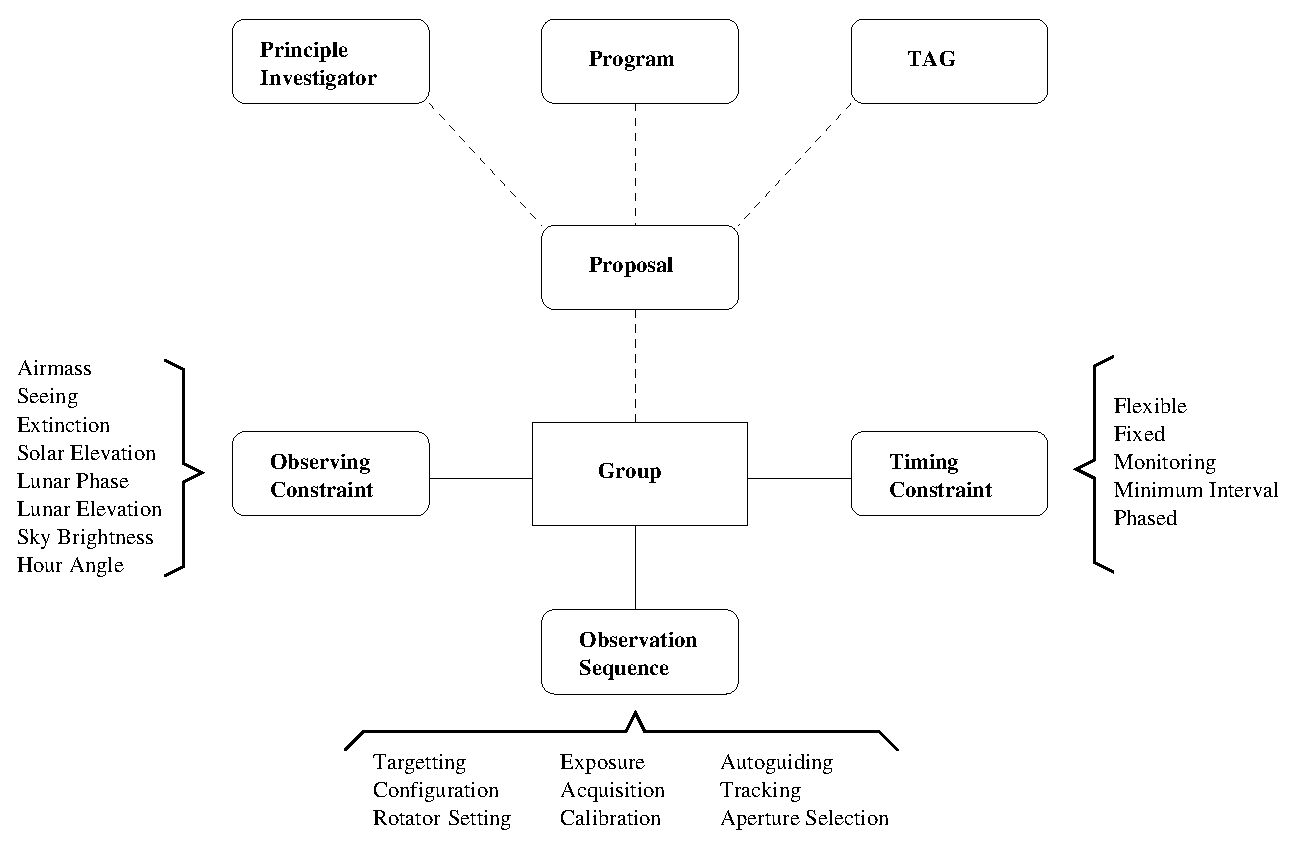
\includegraphics[scale=0.6, angle=0]{figures/group_structure.eps}
  \end{center}
  \caption[Structure of the Phase2 Observing Database (ODB).]
   {Structure of the Phase2 Observing Database (ODB). A \emph{group} contains all the information required to schedule and execute a series of observations. The \emph{observation sequence} contains details of the operations to be performed (target, exposure, instrument selection). \emph{Timing constraints} determine when the group may be executed. \emph{Observing constraints} determine under which atmospheric and other conditions the group is feasible. Groups are contained within a \emph{proposal} containing details of the science program and time allocations from its sponsoring TAG. Each proposal has a \emph{Principle Investigator} who is responsible for entering the observation details  .}
  \label{fig:group}
\end{figure}

% how does the initial OSS work
The current OSS deployed at the telescope \citep{fraser04scheduling} was developed based on the assumption that a despatching scheduler would be best at matching the varying conditions on site with the timing and observing constraints of the available groups. A despatch scheduler works by scanning the set of available groups. Each group which is determined to be feasible (with respect to the current conditions) is assigned a score. Typically, the group with the highest score at that moment in time is then selected for execution.


%\begin{algorithmic}
%\caption{Despatch scheduler algorithm}
%\FORALL{group in ODB} 
%\IF{$feasible(group)$} 
%\STATE $candidates \Leftarrow group$
%\ENDIF
%\ENDFOR

%\REQUIRE $maxscore \gets -99$
%\REQUIRE $best \gets null $
%\FORALL{group in candidates}
%\IF {$score(group) \geq maxscore$}
%\STATE $maxscore \gets score$
%\STATE $best \gets group$
%\ENDIF
%\ENDFOR
%\RETURN best
%\end{algorithmic}

\subsection{Planning and scheduling}
\label{sect:pandstimescales}
The terms planning and scheduling are often confused and indeed used interchangeably. They are however basically different aspects of the same process.
Planning is typically considered to be a long term activity taking a global view of an enterprise. It may set targets or goals to be achieved by the enterprise. These may be somewhat imprecise or abstract - we are not deciding \emph{what} to do and \emph{when} so much as what \emph{sort} of things we want to do and \emph{how well} we want to achieve them. Scheduling on the other hand deals with the rather more precise objective of assigning actual resources to accomplish specific tasks at specific times.

The planning \emph{horizon} is the period over which a plan is made or is expected to be of some utility in achieving its set of goals. In practice we can usefully subdivide planning into several different levels characterized by their horizons \citep{haxhierarchic73}. The subdivisions are by no means set in stone and more or fewer horizons may be more suited to specific enterprises. As we move down the hierarchy, typically, the precision of the objectives becomes more focused and the horizon time span decreases \citep{chien00aspen}.

\begin{description}
\item[Strategic] planning involves the creation of plans to cover very long periods of time. In the current context this could be a semester of telescope time, and more generally could at its most extreme represent the entire lifetime of an enterprise. 
\item[Tactical] plans are designed to cover medium periods e.g. a lunar cycle or half cycle on a telescope,  weekly or monthly production targets in a factory.
\item[Operational] plans \footnote{may also be refered to as \emph{Mission planning}} are short term plans designed to allow an enterprise to function on a day to day basis. Typically they cover the \emph{standard} work-period of the enterprise e.g. a night's observing at a telescope, a shift at a factory.
\item[Scheduling] Takes place over a short period and deals with the specific assignment of resources to tasks. This could range from determination of just the next observation upto the specification of the sequence of observations over the next few hours.
\end{description}

In this thesis we shall consider only the problem of scheduling. Though levels of planning may be incorporated into a final operationally deployed system they are likely to manifest themselves through adjustment of the relative weightings of the quality metrics used by the schedulers over periods longer than a night. 


% e.g. in the form of objective functions or the specification of constraints and preferences to be considered by lower layers. 

\subsection{Motivation}

This system has been in operation now for 7 years since the telescope went on sky (2004) and has performed adequately, however a number of criticisms can be made concerning this implementation.

\begin{itemize}

%\item [obscuration] Due to the objective function scoring mechanism it is not usually clear at any time why a particular group is favored over others or whether a specific group is likely to be selected at a given time. We cannot event tell which group might be selected next.

\item There is no \emph{commonly agreed} mechanism for measuring what represents a \emph{good} schedule (but see \citep{steele97control}). In order to compare the results of different scheduling implementations we need some means of determining the value or reward associated with a schedule. This can be considered from 2 points of view. For the user, the highest reward is likely to be achieved if his observations are made regularly, at the most favourable times with respect to the timing constraints and under the most favourable environmental conditions. For the enterprise, the highest reward might be achieved if the observations selected are most \emph{valuable} in terms of TAG assigned priority and may require some degree of program completeness to be sasified .

\item We do not have a detailed understanding of how conditions change on site and how this might affect planning and scheduling. At present no consideration of environmental change is considered in the planning and scheduling process. Similarly there is no real understanding of the effects on scheduling of the potentially rapidly changing content (volatility) of the ODB.

\item Despatch schedulers have been described as \emph{myopic} \citep{cicirello01random}, in that they select the \emph{best group} to execute at a point in time without reference to what might lead to an overall good schedule. There is no consideration of whether a better sequence might be generated by looking ahead a few steps. This is an example of \emph{local} rather than \emph{global} optimization.
%\item difficult - how do we select the best relative weighting for metrics?.

%\item [efficiency] The current scheduler must be invoked on demand whenever the RCS has completed a group and must then search through the entire ODB to determine which groups are feasible, score these and determine the current best group. 

\end{itemize}

It was therefore decided to conduct a series of experiments using different scheduler paradigms in order to determine how these would perform under a range of environmental and load scenarios.

\subsection{Plan}

The thesis is divided into 2 parts. In the first part, information is gathered to measure and characterize the operating environment and then used to design a scheduling architecture. 

\begin{enumerate}
\item In Sect.~\ref{sect:metrics} an investigation is made into the subject of metrics and reward. Two types of metric are considered. Complexity ($C$) metrics are applied to the measurement of ODB characteristics. These indicate how \emph{difficult} a particular scheduling problem might be. Quality ($Q$) metrics are used to measure the reward or value of a generated schedule and allow a comparision between the success of different scheduler implementations or between different problem sets. 

\item Software embedded within the current robotic control system and scheduler is used to collect information relating to the characteristics of the telescope's operating environment. This information is analysed in Sect.~\ref{sect:character} to determine whether it will be possible to incorporate predictions of environmental conditions into decision making. 

\item Information gathered in the 2 preceding stages is used to design an architecture with which to build a variety of scheduler and planner implementations and incorporating components with which to construct simulation environments to test these schedulers. Heuristic scoring ($f$) metrics are employed by the scheduler and planner implementations to perform search and optimization processes. Mitigation of the effects of changing conditions are considered by looking at the concept of discounted future reward. The scheduler architecture is described in Sect.~\ref{sect:architecture} with further details of the simulation components in Sect.~\ref{sect:experiments}.
\end{enumerate}

In the second part of the thesis a number of simulation experiments are performed using the framework described in Sect.~\ref{sect:architecture}

Two different types of scheduler are considered. The \emph{despatch} scheduler, as currently operationally deployed works by considering which of the various feasible candidates achieves the best score under a particular scoring model at the current time under the current conditions. The \emph{look-ahead} scheduler examines a number of feasible sequences of observations starting from the current time and looking forward by a single horizon length. It compares each sequence selecting the one which maximizes the potential reward.

\begin{enumerate}
\item In Sect.~\ref{sect:mam_study} a human scheduler is pitted against a simple despatch scheduler to act as a shakedown for the framework and to provide a baseline against which to test further schedulers.

\item The effect of varying the weights of the various scoring metrics on schedule quality is tested in Sect.~\ref{sect:exp_scoring}.

\item An investigation into the scale and range of Phase 2 loading is made in Sect.~\ref{sect:exp_complexity}. Schedulers are tested against generated Phase 2 models of differing complexity to determine how this affects scheduling performance.

\item Experiments are performed in Sect.~\ref{sect:exp_stability} to investigate the effect of variable environmental stability on schedulers and to determine which schedulers if any perform best under differing stability regimes.

\item Various unpredicted disruptive events can take place during a night's observing. An investigation into the effects of these disruptive events on schedule quality is made in Sect.~\ref{sect:exp_disruption}.

\item When the content of the Phase 2 ODB is changed during the course of the observing night there is likely to be some effect on scheduling. A detailed study of the effects of Phase 2 volatility are investigated in Sect.~\ref{sect:exp_volatility} in order to determine their effect on scheduling quality.


\item Look-ahead schedulers must decide at some point on how long a forward horizon they should use. In Sect.~\ref{sect:exp_reliability} simulations are performed to investigate how the reliability of determination of such horizon lengths based on environmental stability criteria affects these schedulers.


%\item Develop a despatch scheduler as a baseline with which to test more advanced schedulers, Tune the baseline scheduler using various controllable parameters, typically objective weighting functions and bias function, to investigate the limits of this scheduling paradigm in the telescope scheduling context.

%\item As the basis for the final system, I will develop a look-ahead scheduler incorporating (really !!) short-term prediction of environmental statistics to allow advanced planning of observations and using feedback of performance to adjust the plan objectives.

%\item Investigate variation of scheduling control parameters and horizon length on quality of schedules generated under varying environmental models to determine how to adapt to these - teh quality of schedules generated will be compared to those geenrated by the baseline system working at its maximum efficiency.

%\item Knowledge gained from this investigation will be incorporated into a final adaptive, look-ahead scheduler.
\end{enumerate}


\end{document}
